\documentclass{article}
\usepackage{fancyhdr}
\usepackage{amsthm}
\usepackage{etoolbox}
\usepackage{verbatim}
\usepackage{enumerate}
\usepackage{amsmath}
\usepackage{algorithmicx}
\usepackage{algorithm}
\usepackage{algpseudocode}
\usepackage{tikz}


	
\pagestyle{fancy}
\title{Chapter 13}
\author{Michelle Bodnar, Andrew Lohr}

\newcounter{curnum}
\setcounter{curnum}{0}

\newtheorem{th1}{Exercise}
\newcommand{\calH}{\mathcal{H}}
\newcommand{\calX}{\mathcal{X}}
\newcommand{\calA}{\mathcal{A}}
\newcommand{\calY}{\mathcal{Y}}

\begin{document}
\maketitle

\noindent\textbf{ Exercise 13.1-1} \\

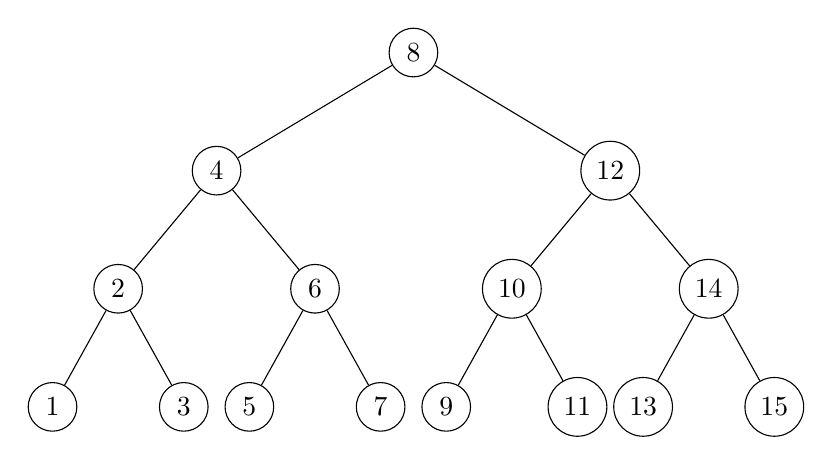
\begin{tikzpicture}[level/.style={sibling distance=50mm/#1}]
\node [circle,draw] (a){8}
  child {
  node [circle,draw] (b) {4}
    child {
    node [circle,draw] (c) {2}
        child {
            node [circle,draw] (d) {1}
        }
            child {
                node [circle,draw] (e) {3}
            }
      }
    child {
    node [circle,draw] (f) {6}
        child {
            node [circle,draw] (g) {5}
        }
            child {
                node [circle,draw] (h) {7}
            }
  }
  }
  child {
  node [circle,draw] (i) {12}
    child {
    node [circle,draw] (j) {10}
        child {
            node [circle,draw] (k) {9}
        }
            child {
                node [circle,draw] (l) {11}
            }
      }
    child {
    node [circle,draw] (m) {14}
        child {
            node [circle,draw] (n) {13}
        }
            child {
                node [circle,draw] (o) {15}
            }
  }
  };
\end{tikzpicture}

We shorten NIL to N so that it can be more easily displayed in the document. The following has black height 2.

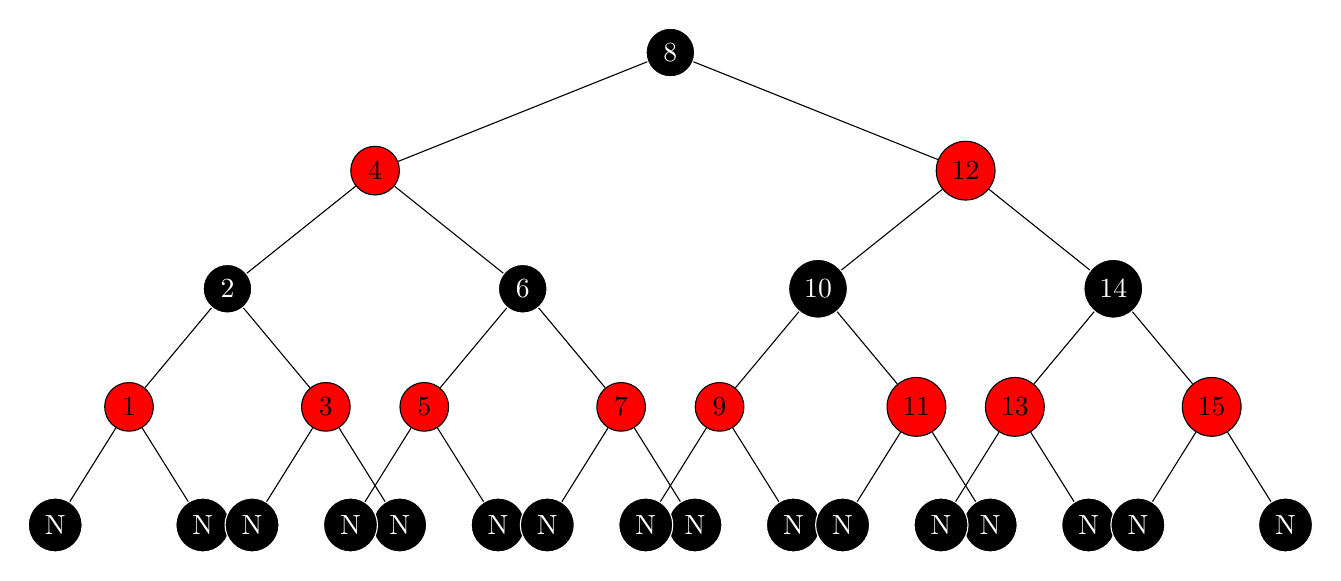
\begin{tikzpicture}[level/.style={sibling distance=75mm/#1}]
\node [circle,draw,color=white, fill=black] (a){8}
  child {
  node [circle,draw,fill =red] (b) {4}
    child {
    node [circle,draw,color=white, fill=black] (c) {2}
        child {
            node [circle,draw,fill =red] (d) {1}
            child{node [circle,draw,color=white, fill=black] (p) {N}}
            child{node [circle,draw,color=white, fill=black] (q) {N}}
        }
            child {
                node [circle,draw,fill =red] (e) {3}
            child{node [circle,draw,color=white, fill=black] (r) {N}}
            child{node [circle,draw,color=white, fill=black] (s) {N}}
            }
      }
    child {
    node [circle,draw,color=white, fill=black] (f) {6}
        child {
            node [circle,draw,fill =red] (g) {5}
            child{node [circle,draw,color=white, fill=black] (t) {N}}
            child{node [circle,draw,color=white, fill=black] (u) {N}}
        }
            child {
                node [circle,draw,fill =red] (h) {7}
            child{node [circle,draw,color=white, fill=black] (v) {N}}
            child{node [circle,draw,color=white, fill=black] (w) {N}}
            }
  }
  }
  child {
  node [circle,draw,fill =red] (i) {12}
    child {
    node [circle,draw,color=white, fill=black] (j) {10}
        child {
            node [circle,draw,fill =red] (k) {9}
            child{node [circle,draw,color=white, fill=black] (x) {N}}
            child{node [circle,draw,color=white, fill=black] (y) {N}}
        }
            child {
                node [circle,draw,fill =red] (l) {11}
            child{node [circle,draw,color=white, fill=black] (z) {N}}
            child{node [circle,draw,color=white, fill=black] (aa) {N}}
            }
      }
    child {
    node [circle,draw,color=white, fill=black] (m) {14}
        child {
            node [circle,draw,fill =red] (n) {13}
            child{node [circle,draw,color=white, fill=black] (ab) {N}}
            child{node [circle,draw,color=white, fill=black] (ac) {N}}
        }
            child {
                node [circle,draw,fill =red] (o) {15}
            child{node [circle,draw,color=white, fill=black] (ad) {N}}
            child{node [circle,draw,color=white, fill=black] (ae) {N}}
            }
  }
  };
\end{tikzpicture}

The following has black height 3

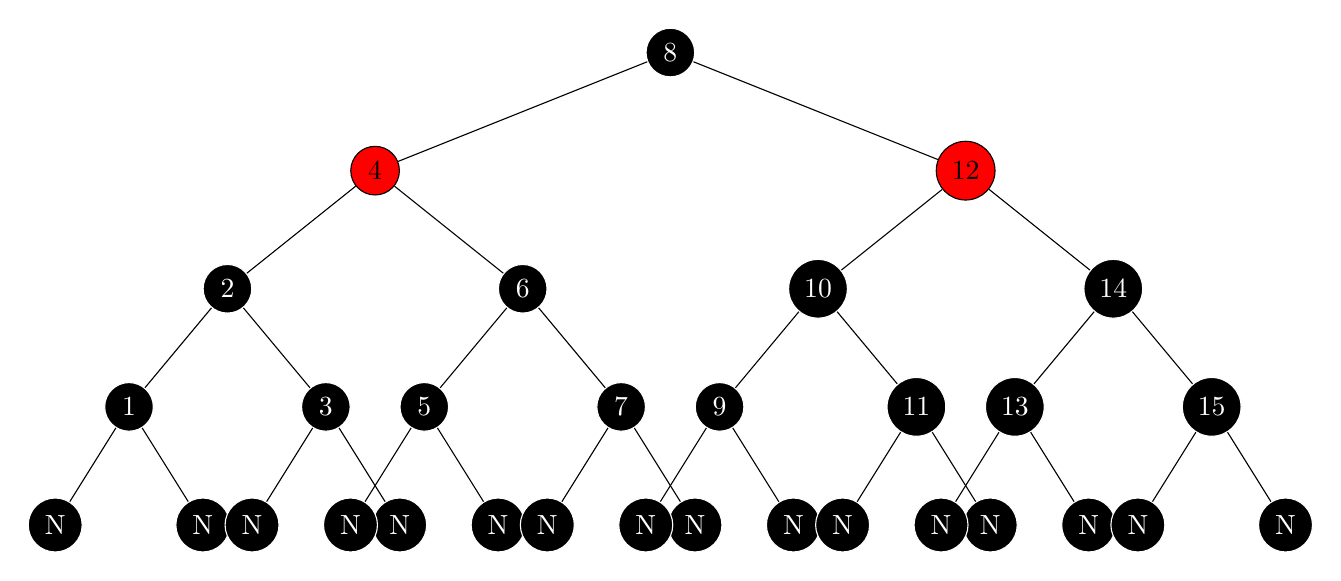
\begin{tikzpicture}[level/.style={sibling distance=75mm/#1}]
\node [circle,draw,color=white, fill=black] (a){8}
  child {
  node [circle,draw,fill =red] (b) {4}
    child {
    node [circle,draw,color=white, fill=black] (c) {2}
        child {
            node [circle,draw,color=white, fill=black] (d) {1}
            child{node [circle,draw,color=white, fill=black] (p) {N}}
            child{node [circle,draw,color=white, fill=black] (q) {N}}
        }
            child {
                node [circle,draw,color=white, fill=black] (e) {3}
            child{node [circle,draw,color=white, fill=black] (r) {N}}
            child{node [circle,draw,color=white, fill=black] (s) {N}}
            }
      }
    child {
    node [circle,draw,color=white, fill=black] (f) {6}
        child {
            node [circle,draw,color=white, fill=black] (g) {5}
            child{node [circle,draw,color=white, fill=black] (t) {N}}
            child{node [circle,draw,color=white, fill=black] (u) {N}}
        }
            child {
                node [circle,draw,color=white, fill=black] (h) {7}
            child{node [circle,draw,color=white, fill=black] (v) {N}}
            child{node [circle,draw,color=white, fill=black] (w) {N}}
            }
  }
  }
  child {
  node [circle,draw,fill =red] (i) {12}
    child {
    node [circle,draw,color=white, fill=black] (j) {10}
        child {
            node [circle,draw,color=white, fill=black] (k) {9}
            child{node [circle,draw,color=white, fill=black] (x) {N}}
            child{node [circle,draw,color=white, fill=black] (y) {N}}
        }
            child {
                node [circle,draw,color=white, fill=black] (l) {11}
            child{node [circle,draw,color=white, fill=black] (z) {N}}
            child{node [circle,draw,color=white, fill=black] (aa) {N}}
            }
      }
    child {
    node [circle,draw,color=white, fill=black] (m) {14}
        child {
            node [circle,draw,color=white, fill=black] (n) {13}
            child{node [circle,draw,color=white, fill=black] (ab) {N}}
            child{node [circle,draw,color=white, fill=black] (ac) {N}}
        }
            child {
                node [circle,draw,color=white, fill=black] (o) {15}
            child{node [circle,draw,color=white, fill=black] (ad) {N}}
            child{node [circle,draw,color=white, fill=black] (ae) {N}}
            }
  }
  };
\end{tikzpicture}

Lastly, the following has black height 4.

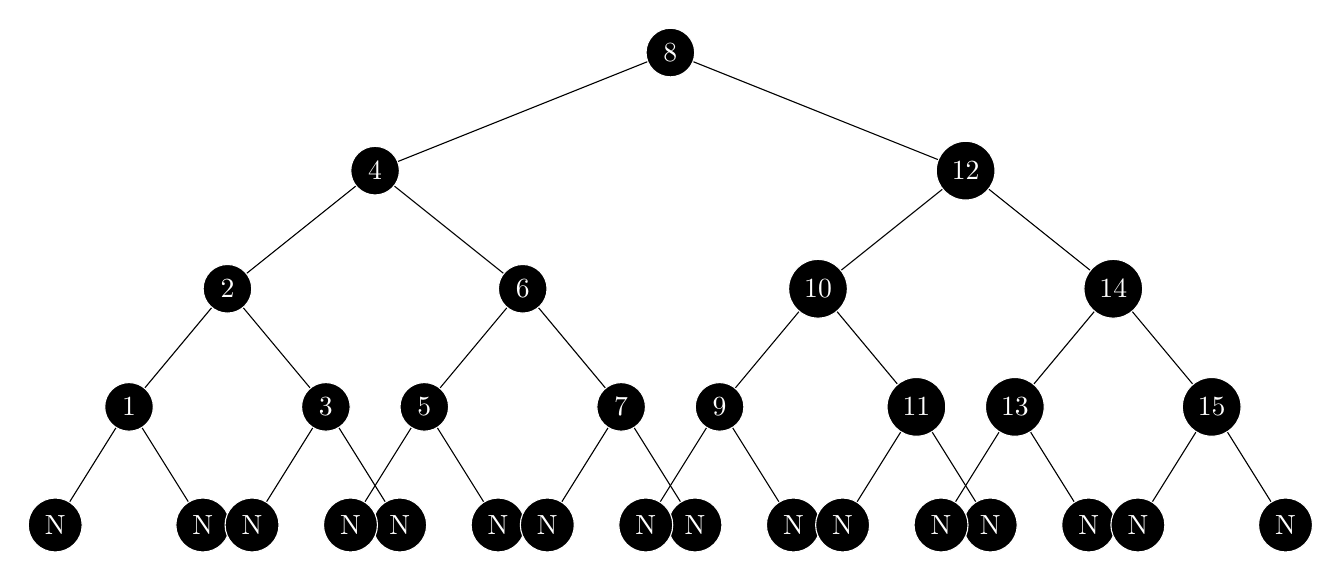
\begin{tikzpicture}[level/.style={sibling distance=75mm/#1}]
\node [circle,draw,color=white, fill=black] (a){8}
  child {
  node [circle,draw,color=white, fill=black] (b) {4}
    child {
    node [circle,draw,color=white, fill=black] (c) {2}
        child {
            node [circle,draw,color=white, fill=black] (d) {1}
            child{node [circle,draw,color=white, fill=black] (p) {N}}
            child{node [circle,draw,color=white, fill=black] (q) {N}}
        }
            child {
                node [circle,draw,color=white, fill=black] (e) {3}
            child{node [circle,draw,color=white, fill=black] (r) {N}}
            child{node [circle,draw,color=white, fill=black] (s) {N}}
            }
      }
    child {
    node [circle,draw,color=white, fill=black] (f) {6}
        child {
            node [circle,draw,color=white, fill=black] (g) {5}
            child{node [circle,draw,color=white, fill=black] (t) {N}}
            child{node [circle,draw,color=white, fill=black] (u) {N}}
        }
            child {
                node [circle,draw,color=white, fill=black] (h) {7}
            child{node [circle,draw,color=white, fill=black] (v) {N}}
            child{node [circle,draw,color=white, fill=black] (w) {N}}
            }
  }
  }
  child {
  node [circle,draw,color=white, fill=black] (i) {12}
    child {
    node [circle,draw,color=white, fill=black] (j) {10}
        child {
            node [circle,draw,color=white, fill=black] (k) {9}
            child{node [circle,draw,color=white, fill=black] (x) {N}}
            child{node [circle,draw,color=white, fill=black] (y) {N}}
        }
            child {
                node [circle,draw,color=white, fill=black] (l) {11}
            child{node [circle,draw,color=white, fill=black] (z) {N}}
            child{node [circle,draw,color=white, fill=black] (aa) {N}}
            }
      }
    child {
    node [circle,draw,color=white, fill=black] (m) {14}
        child {
            node [circle,draw,color=white, fill=black] (n) {13}
            child{node [circle,draw,color=white, fill=black] (ab) {N}}
            child{node [circle,draw,color=white, fill=black] (ac) {N}}
        }
            child {
                node [circle,draw,color=white, fill=black] (o) {15}
            child{node [circle,draw,color=white, fill=black] (ad) {N}}
            child{node [circle,draw,color=white, fill=black] (ae) {N}}
            }
  }
  };
\end{tikzpicture}\\

\noindent\textbf{Exercise 13.1-2}\\

If the inserted node is red then it won't be a red-black tree because 35 will be the parent of 36, which is also colored red.  If the inserted node is black it will also fail to be a red-black tree because there will be two paths from node 38 to T.nil which contain different numbers of black nodes, violating property 5. In the picture of the tree below, the NIL nodes have been omitted for space reasons.


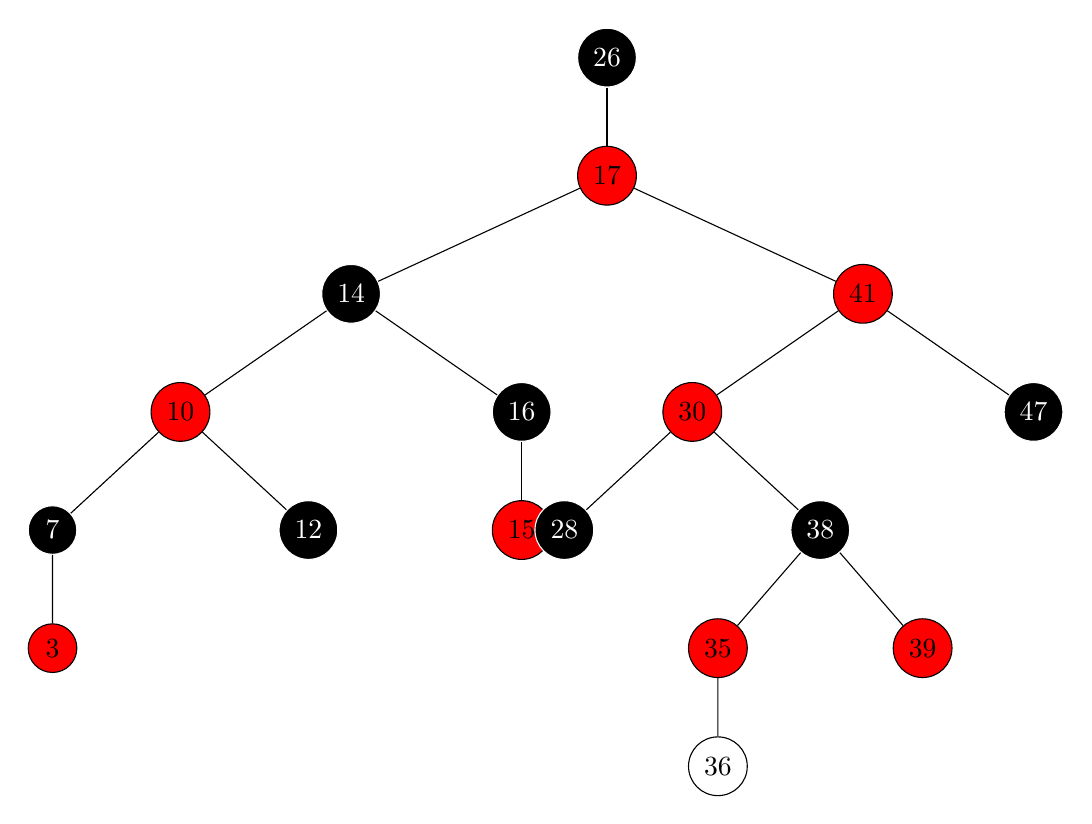
\begin{tikzpicture}[level/.style={sibling distance=130mm/#1}]
\node [circle,draw,color=white, fill=black] (a){26}
child {node [circle,draw,fill =red] (b) {17}
	child {node [circle,draw,color=white, fill=black] (c) {14}
       		child {node [circle,draw,fill =red] (d) {10}
			child{node [circle,draw,color = white,fill =black] (e) {7}
				child {node [circle,draw,fill =red] (f) {3}}
			}
			child{node [circle,draw,color = white,fill =black] (g) {12}}
		}
            	child {node [circle,draw,color = white,fill =black] (h) {16}
			child{node [circle,draw,color = black,fill =red] (i) {15}}
           		 }
		}
	child{node [circle,draw,color = black,fill =red] (j) {41}
		child{node [circle,draw,color = black,fill =red] (k) {30}
			child{node [circle,draw,color = white,fill =black] (l) {28}}
			child{node [circle,draw,color = white,fill =black] (m) {38}
				child{node [circle,draw,color = black,fill =red] (n) {35}
					child{node [circle,draw,color = black] (l) {36}}
				}
				child{node [circle,draw,color = black,fill =red] (o) {39}}
			}
		}
		child{node [circle,draw,color = white,fill =black] (p) {47}}
	}
};
\end{tikzpicture}

\noindent\textbf{ Exercise 13.1-3} \\

It will. There was no red node introduced, so 4 will still be satisfied. Since the root is in every path from the root to the leaves, but no others. 5 will be satisfied because the only paths we will be changing the number of black nodes in are those coming from the root. All of these will increase by 1, and so will all be equal. 3 is trivially preserved, as no new leaves are introduced. 1 is also trivially preserved as only one node is changed and it is not changed to some mysterious third color.\\

\noindent\textbf{Exercise 13.1-4}\\

The possible degrees are 0 through 5, based on whether or not the black node was a root and whether it had one or two red children, each with either one or two black children. The depths could shrink by at most a factor of 1/2. \\

\noindent\textbf{ Exercise 13.1-5} \\

Suppose we have the longest simple path $(a_1,a_2,\ldots a_s)$ and the shortest simple path $(b_1,b_2, \ldots, b_t)$. Then, by property 5 we know they have equal numbers of black nodes. By property 4, we know that neither contains a repeated red node. This tells us that at most $\lfloor\frac{s-1}{2}\rfloor$ of the nodes in the longest path are red. This means that at least $\lceil \frac{s+1}{2} \rceil$ are black, so, $t\ge \lceil \frac{s+1}{2} \rceil$. So, if, by way of contradiction, we had that $s>t*2$, then $  t \ge \lceil \frac{s+1}{2} \rceil \ge \lceil\frac{2t+2}{2} \rceil = t+1$ a contradiction.\\

\noindent\textbf{Exercise 13.1-6}\\

In a path from root to leaf we can have at most one red node between any two black nodes, so maximal height of such a tree is $2k+1$, where each path from root to leaf is alternating red and black nodes. To maximize internal nodes, we make the tree complete, giving a total of $2^{2k+1} - 1$ internal nodes. The smallest possible number of internal nodes comes from a complete binary tree, where every node is black.  This has $2^{k+1} - 1$ internal nodes. \\

\noindent\textbf{ Exercise 13.1-7} \\

Since each red node needs to have two black children, our only hope at getting a large number of internal red nodes relative to our number of black internal nodes is to make it so that the parent of every leaf is a red node. So, we would have a ratio of $\frac{2}{3}$ if we have the tree with a black root which has red children, and all of it's grandchildren be leaves. We can't do better than this because as we make the tree bigger, the ratio approaches $\frac{1}{2}$.

The smallest ratio is achieved by having a complete tree that is balanced and black as a raven's feather. For example, see the last tree presented in the solution to 13.1-1. \\

\noindent\textbf{ Exercise 13.2-1} \\

See the algorithm for RIGHT-ROTATE.\\


\begin{algorithm}
\caption{RIGHT-ROTATE(T,x)}
\begin{algorithmic}
\State y = x.left
\State x.left = y.right
\If{$y.right \neq T.nil$}
\State t.right.p = x
\EndIf
\State y.p = x.p
\If{x.p == T.nil}
\State T.root = y
\ElsIf{x == x.p.left}
\State x.p.left = y
\Else
\State x.p.right = y
\EndIf
\State y.right =x
\State x.p =y
\end{algorithmic}
\end{algorithm}

\noindent\textbf{Exercise 13.2-2}\\

We proceed by induction.  In a tree with only one node, the root has neither a left nor a right child, so no rotations are valid.  Suppose that a tree on $n\geq 0$ nodes has exactly $n-1$ rotations.  Let $T$ be a binary search tree on $n+1$ nodes.  If $T.root$ has no right child then the root can only be involved in a right rotation, and the left child of $T$ has $n$ vertices, so it has exactly $n-1$ rotations, yielding a total of $n$ for the whole tree.  The argument is identical if $T.root$ has no left child.  Finally, suppose $T.root$ has two children, and let $k$ denote the number of nodes in the left subtree.  Then the root can be either left or right rotated, contributing 2 to the count.  By the induction hypothesis, $T.left$ has exactly $k-1$ rotations and $T.right$ has exactly $n-k-1-1$ rotations, so there are a total of $2 + k-1 + n-k-1-1 = n$ possible rotations, completing the proof. \\

\noindent\textbf{ Exercise 13.2-3} \\

the depth of $c$ decreases by one, the depth of $b$ stays the same, and the depth of $a$ increases by 1.\\

\noindent\textbf{Exercise 13.2-4}\\

Consider transforming an arbitrary $n$-node BT into a right-going chain as follows: Let the root and all successive right children of the root be the elements of the chain initial chain.  For any node $x$ which is a left child of a node on the chain, a single right rotation on the parent of $x$ will add that node to the chain and not remove any elements from the chain.  Thus, we can convert any BST to a right chain with at most $n-1$ right rotations.  Let $r_1, r_2, \ldots, r_k$ be the sequence of rotations required to convert some BST $T_1$ into a right-going chain, and let $s_1, s_2, \ldots, s_m$ be the sequence of rotations required to convert some other BST $T_2$ to a right-going chain.  Then $k < n$ and $m < n$, and we can convert $T_1$ to $T_2$ be performing the sequence $r_1, r_2, \ldots, r_k, s_m' s_{m-1}', \ldots, s_1'$ where $s_i'$ is the opposite rotation of $s_i$.  Since $k+m < 2n$, the number of rotations required is $O(n)$. \\

\noindent\textbf{ Exercise 13.2-5} \\

Consider the BST for $T_2$ to be

\begin{tikzpicture}[level/.style={sibling distance=75mm/#1}]
\node [circle,draw] (a){8}
  child {
  node [circle,draw] (b) {4}
    child {node [circle,draw] (c) {NIL}
    }
      child {node [circle,draw] (d) {NIL}
      }
  }
  child{ node [circle,draw] (e) {NIL}};
\end{tikzpicture}

And let $T_1$ be 

    \begin{tikzpicture}[level/.style={sibling distance=75mm/#1}]
\node [circle,draw] (a){8}
  child{ node [circle,draw] (e) {NIL}}
  child {
  node [circle,draw] (b) {4}
    child {node [circle,draw] (c) {NIL}
    }
      child {node [circle,draw] (d) {NIL}
      }
  };
\end{tikzpicture}

Then, there are no nodes for which its valid to call right rotate in $T_1$. Even though it is possible to right convert $T_2$ into $T_1$, the reverse is not possible.


For any BST T, define the quantity $f(T)$ to be the sum over all the nodes of the number of left pointers that are used in a simple path from the root to that node. Note that the contribution from each node is $O(n)$. Since there are only $n$ nodes, we have that $f(T)$ is $O(n^2)$. Also, when we call RIGHT-ROTATE(T,x), then the contribution from $x$ decreases by one, and the contribution from all other elements remain the same. Since $f(T)$ is a quantity that decreases by exactly one with every call of RIGHT-ROTATE, and begins $O(n^2)$, and never goes negative, we know that there can only be at most $O(n^2)$ calls of RIGHT-ROTATE on a BST.\\



\noindent\textbf{ Exercise 13.3-1} \\

If we chose to set the color of $z$ to black then we would be violating property 5 of being a red-black tree. Because any path from the root to a leaf under $z$ would have one more black node than the paths to the other leaves \\

\noindent\textbf{Exercise 13.3-2}\\
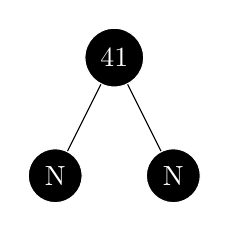
\begin{tikzpicture}
\node [circle,draw,color=white, fill=black] (a){41}
	child{node [circle,draw,color=white, fill=black] (b) {N}}
	child{node [circle,draw,color=white, fill=black] (c) {N}};
\end{tikzpicture}

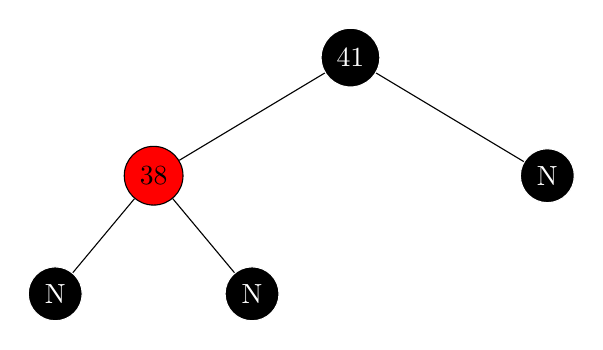
\begin{tikzpicture}[level/.style={sibling distance=50mm/#1}]
\node [circle,draw,color=white, fill=black] (a){41}
child{node [circle,draw,fill =red] (b) {38}
	child{node [circle,draw,color=white, fill=black] (c) {N}}
	child{node [circle,draw,color=white, fill=black] (d) {N}}}
child{node [circle,draw,color=white, fill=black] (e) {N}};
\end{tikzpicture}

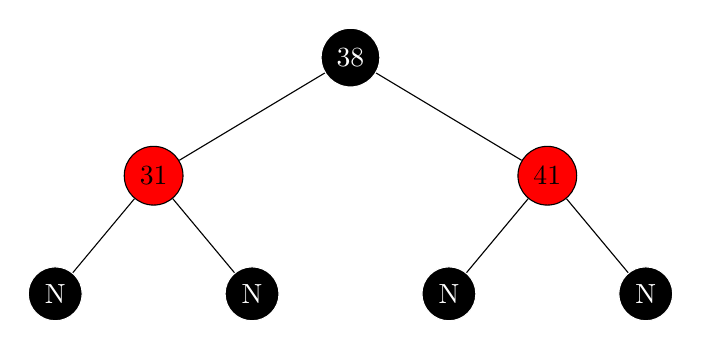
\begin{tikzpicture}[level/.style={sibling distance=50mm/#1}]
\node [circle,draw,color=white, fill=black] (a){38}
	child{node [circle,draw,color=black, fill=red] (b) {31}
		child{node [circle,draw,color=white, fill=black] (c) {N}}
		child{node [circle,draw,color=white, fill=black] (d) {N}}}
	child{node [circle,draw,color=black, fill=red] (e) {41}
		child{node [circle,draw,color=white, fill=black] (f) {N}}
		child{node [circle,draw,color=white, fill=black] (g) {N}}};
\end{tikzpicture}

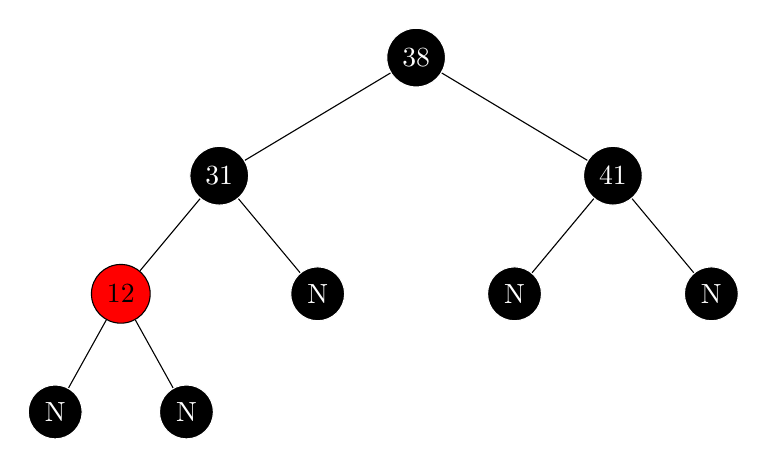
\begin{tikzpicture}[level/.style={sibling distance=50mm/#1}]
\node [circle,draw,color=white, fill=black] (a){38}
	child{node [circle,draw,color=white, fill=black] (b) {31}
		child{node [circle,draw,color=black, fill=red] (c) {12}
			child{node [circle,draw,color=white, fill=black] (h) {N}}
			child{node [circle,draw,color=white, fill=black] (i) {N}}}
		child{node [circle,draw,color=white, fill=black] (d) {N}}}
	child{node [circle,draw,color=white, fill=black] (e) {41}
		child{node [circle,draw,color=white, fill=black] (f) {N}}
		child{node [circle,draw,color=white, fill=black] (g) {N}}};
\end{tikzpicture}

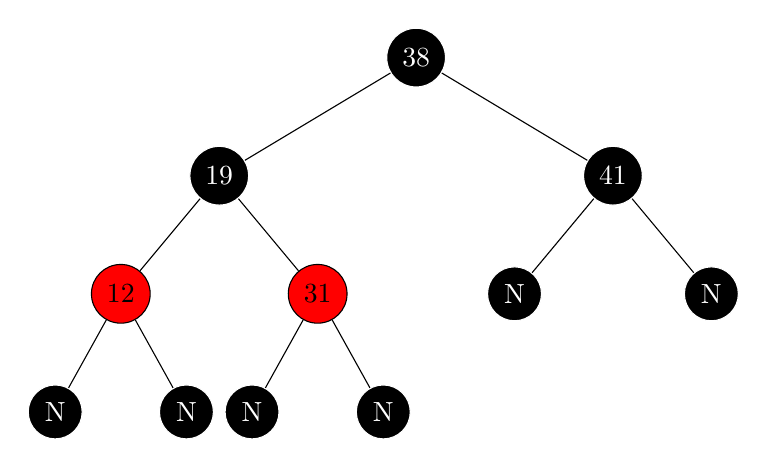
\begin{tikzpicture}[level/.style={sibling distance=50mm/#1}]
\node [circle,draw,color=white, fill=black] (a){38}
	child{node [circle,draw,color=white, fill=black] (b) {19}
		child{node [circle,draw,color=black, fill=red] (c) {12}
			child{node [circle,draw,color=white, fill=black] (h) {N}}
			child{node [circle,draw,color=white, fill=black] (i) {N}}}
		child{node [circle,draw,color=black, fill=red] (d) {31}
			child{node [circle,draw,color=white, fill=black] (j) {N}}
			child{node [circle,draw,color=white, fill=black] (k) {N}}}}
	child{node [circle,draw,color=white, fill=black] (e) {41}
		child{node [circle,draw,color=white, fill=black] (f) {N}}
		child{node [circle,draw,color=white, fill=black] (g) {N}}};
\end{tikzpicture}

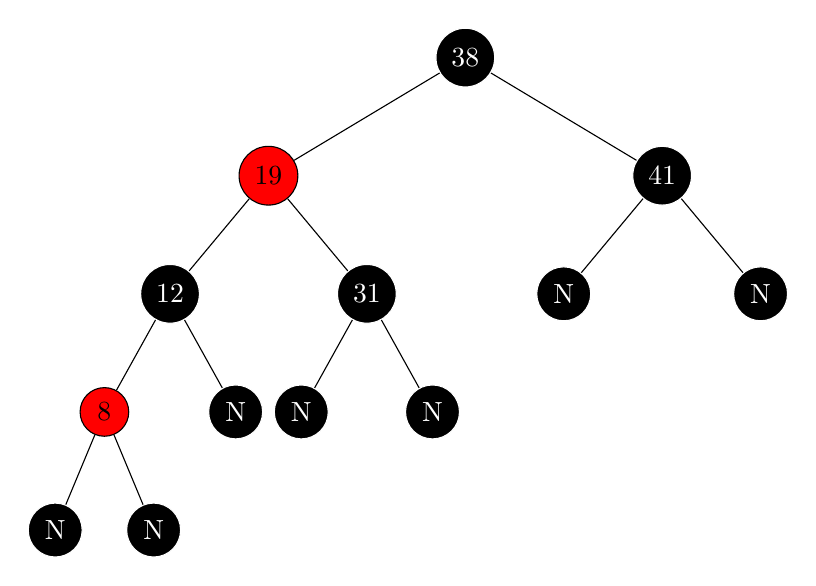
\begin{tikzpicture}[level/.style={sibling distance=50mm/#1}]
\node [circle,draw,color=white, fill=black] (a){38}
	child{node [circle,draw,color=black, fill=red] (b) {19}
		child{node [circle,draw,color=white, fill=black] (c) {12}
			child{node [circle,draw,color=black, fill=red] (h) {8}
				child{node [circle,draw,color=white, fill=black] (l) {N}}
				child{node [circle,draw,color=white, fill=black] (m) {N}}}
			child{node [circle,draw,color=white, fill=black] (i) {N}}}
		child{node [circle,draw,color=white, fill=black] (d) {31}
			child{node [circle,draw,color=white, fill=black] (j) {N}}
			child{node [circle,draw,color=white, fill=black] (k) {N}}}}
	child{node [circle,draw,color=white, fill=black] (e) {41}
		child{node [circle,draw,color=white, fill=black] (f) {N}}
		child{node [circle,draw,color=white, fill=black] (g) {N}}};
\end{tikzpicture}\\


\noindent\textbf{ Exercise 13.3-3} \\

For the z being a right child case, we append the black height of each node to get
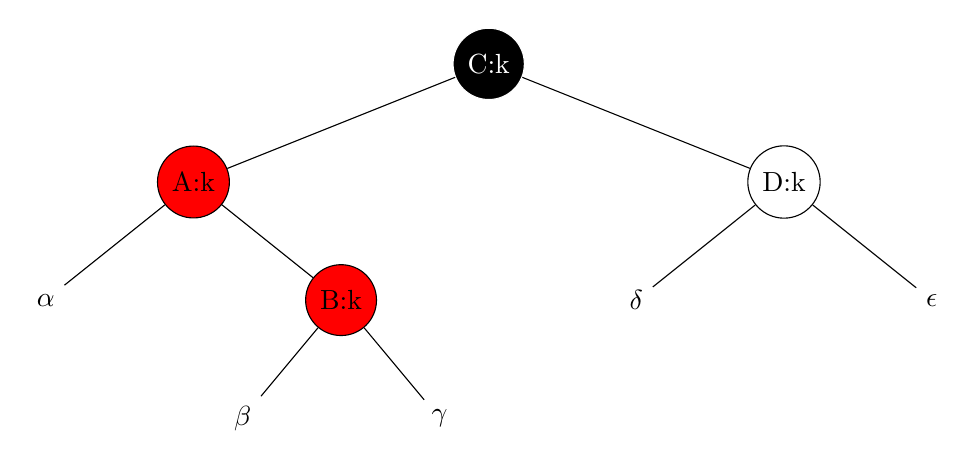
\begin{tikzpicture}[level/.style={sibling distance=75mm/#1}]
\node [circle,draw,color=white, fill=black] (a){C:k}
  child{ node [circle,draw,fill=red] (e) {A:k} 
  child{node (z){$\alpha$}}
  child{node[circle,draw,fill=red] (y) {B:k} 
  child{node  (x){$\beta$}}
  child{node (w){$\gamma$}
  }
  }}
  child {
  node [circle,draw] (b) {D:k}
    child {node  (c){$\delta$}
    }
      child {node (d){$\epsilon$}
      }
  };
\end{tikzpicture}

which goes to

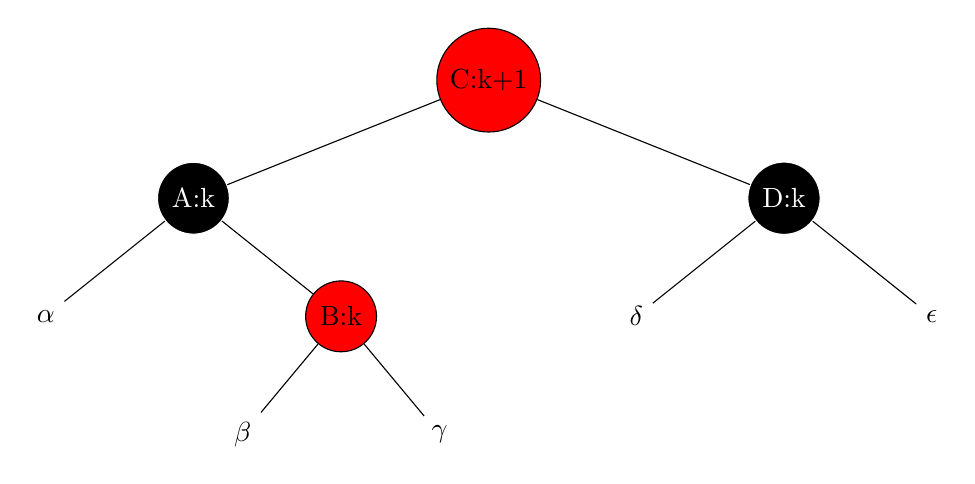
\begin{tikzpicture}[level/.style={sibling distance=75mm/#1}]
\node [circle,draw,fill=red] (a){C:k+1}
  child{ node [circle,draw,color=white, fill=black] (e) {A:k} 
  child{node (z){$\alpha$}}
  child{node[circle,draw,fill=red] (y) {B:k} 
  child{node  (x){$\beta$}}
  child{node (w){$\gamma$}
  }
  }}
  child {
  node [circle,draw,color=white, fill=black] (b) {D:k}
    child {node  (c){$\delta$}
    }
      child {node (d){$\epsilon$}
      }
  };
\end{tikzpicture}

note that while the black depths of the nodes may of changed, they are still well defined, and so they still satisfy condition 5 of being a red-black tree. Similar trees for when z is a left child.\\

\noindent\textbf{Exercise 13.3-4}\\

First observe that RB-INSERT-FIXUP only modifies the child of a node if it is already red, so we will never modify a child which is set to $T.nil$.  We just need to check that the parent of the root is never set to red. Since the root and the parent of the root are automatically black, if $z$ is at depth less than 2, the while loop will be broken.  We only modify colors of nodes at most two levels above $z$, so the only case we need to worry about is if $z$ is at depth 2.  In this case we risk modifying the root to be red, but this is handled in line 16.  When $z$ is updated, it will either the root or the child of the root. Either way, the root and the parent of the root are still black, so the while condition is violated, making it impossibly to modify $T.nil$ to be red. \\

\noindent\textbf{ Exercise 13.3-5} \\

Suppose we just added the last element. Then, prior to calling RB-INSERT-FIXUP, we have that it is red. In all of the fixup cases for an execution of the while loop, we have that the resulting tree fragment contains a red non-root node. This node will not be later made black on line 16 because it isn't the root. \\

\noindent\textbf{Exercise 13.3-6}\\

We need to remove line 8 from RB-INSERT and modify RB-INSERT-FIXUP.  At any point in RB-INSERT-FIXUP we need only keep track of at most 2 ancestors: $z.p$ and $z.p.p$.  We can find and store each of these nodes in $\log n$ time and use them for the duration of the call to RB-INSERT-FIXUP.  This won't change the running time of RB-INSERT.\\

\noindent\textbf{ Exercise 13.4-1} \\

There are two ways we may of left the while loop of RB-DELETE-FIXUP. The first is that we had $x = T.root$. In this case, we set $x.color = BLACK$ on line 23. So, we must have that the root is black. The other case is that we ended the while loop because we had $x.color == RED$, but had that $x\neq T.root$. This rules out case 4, because that has us setting $x=T.root$. In case 3, we don't set $x$ to be red, or change $x$ at all, so it couldn't of been the last case run. In case 2, we set nothing new to be $RED$, so this couldn't lead to exiting the while loop for this reason. In case 1, we make the sibling black and rotate it into the position of the parent. So, it wouldn't be possible to make the root red in this step because the only node we set to be red, we then placed a black node above. 

\noindent\textbf{Exercise 13.4-2}\\

Suppose that both $x$ and $x.p$ are red in RB-DELETE.  This can only happen in the else-case of line 9.  Since we are deleting from a red-black tree, the other child of $y.p$ which becomes $x's$ sibling in the call to RB-TRANSPLANT on line 14 must be black, so $x$ is the only child of $x.p$ which is red.  The while-loop condition of RB-DELETE-FIXUP(T,x) is immediately violated so we simply set $x.color = black$, restoring property 4. \\

\noindent\textbf{ Exercise 13.4-3} \\

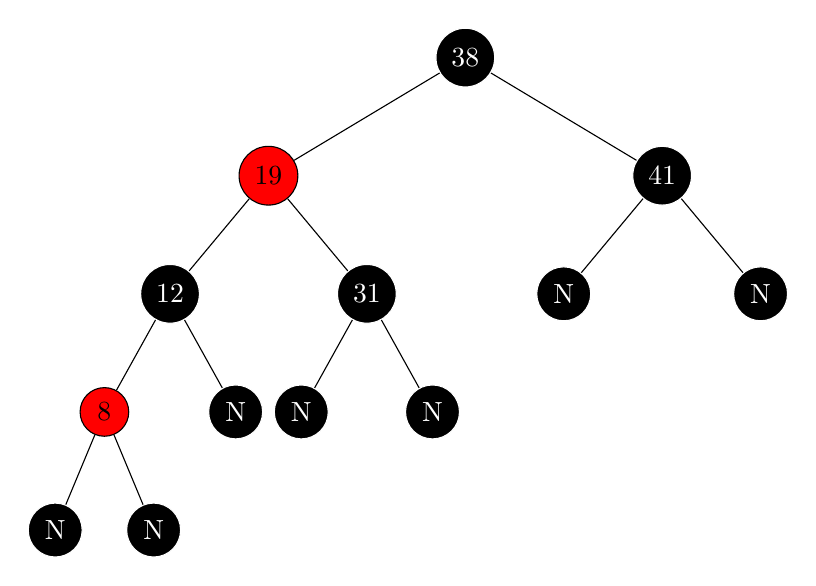
\begin{tikzpicture}[level/.style={sibling distance=50mm/#1}]
\node [circle,draw,color=white, fill=black] (a){38}
	child{node [circle,draw,color=black, fill=red] (b) {19}
		child{node [circle,draw,color=white, fill=black] (c) {12}
			child{node [circle,draw,color=black, fill=red] (h) {8}
				child{node [circle,draw,color=white, fill=black] (l) {N}}
				child{node [circle,draw,color=white, fill=black] (m) {N}}}
			child{node [circle,draw,color=white, fill=black] (i) {N}}}
		child{node [circle,draw,color=white, fill=black] (d) {31}
			child{node [circle,draw,color=white, fill=black] (j) {N}}
			child{node [circle,draw,color=white, fill=black] (k) {N}}}}
	child{node [circle,draw,color=white, fill=black] (e) {41}
		child{node [circle,draw,color=white, fill=black] (f) {N}}
		child{node [circle,draw,color=white, fill=black] (g) {N}}};
\end{tikzpicture}\\

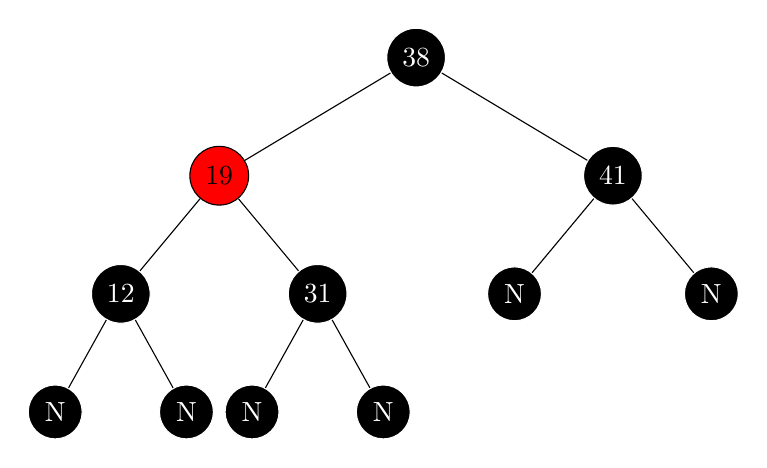
\begin{tikzpicture}[level/.style={sibling distance=50mm/#1}]
\node [circle,draw,color=white, fill=black] (a){38}
	child{node [circle,draw,color=black, fill=red] (b) {19}
		child{node [circle,draw,color=white, fill=black] (c) {12}
			child{node [circle,draw,color=white, fill=black] (l) {N}}
			child{node [circle,draw,color=white, fill=black] (i) {N}}}
		child{node [circle,draw,color=white, fill=black] (d) {31}
			child{node [circle,draw,color=white, fill=black] (j) {N}}
			child{node [circle,draw,color=white, fill=black] (k) {N}}}}
	child{node [circle,draw,color=white, fill=black] (e) {41}
		child{node [circle,draw,color=white, fill=black] (f) {N}}
		child{node [circle,draw,color=white, fill=black] (g) {N}}};
\end{tikzpicture}\\

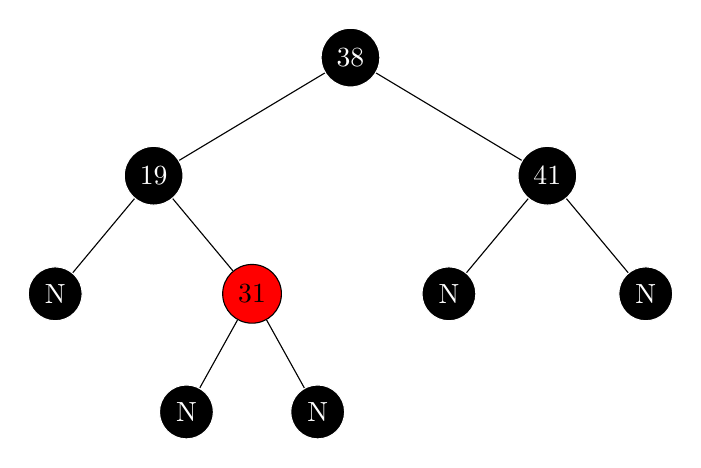
\begin{tikzpicture}[level/.style={sibling distance=50mm/#1}]
\node [circle,draw,color=white, fill=black] (a){38}
	child{node [circle,draw,color=white, fill=black] (b) {19}
		child{node [circle,draw,color=white, fill=black] (i) {N}}
		child{node [circle,draw,color=black, fill=red] (d) {31}
			child{node [circle,draw,color=white, fill=black] (j) {N}}
			child{node [circle,draw,color=white, fill=black] (k) {N}}}}
	child{node [circle,draw,color=white, fill=black] (e) {41}
		child{node [circle,draw,color=white, fill=black] (f) {N}}
		child{node [circle,draw,color=white, fill=black] (g) {N}}};
\end{tikzpicture}\\

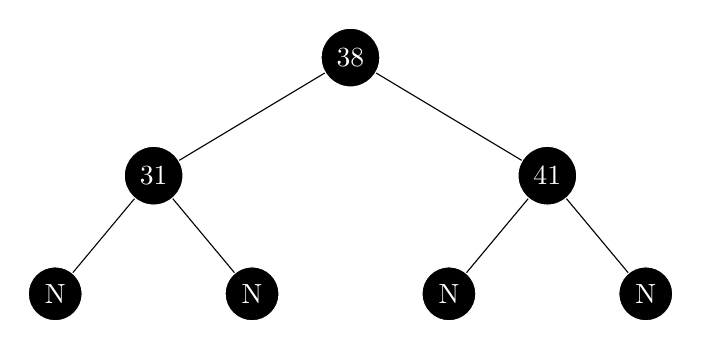
\begin{tikzpicture}[level/.style={sibling distance=50mm/#1}]
\node [circle,draw,color=white, fill=black] (a){38}
	child{node [circle,draw,color=white, fill=black] (b) {31}
		child{node [circle,draw,color=white, fill=black] (i) {N}}
		child{node [circle,draw,color=white, fill=black] (k) {N}}}
	child{node [circle,draw,color=white, fill=black] (e) {41}
		child{node [circle,draw,color=white, fill=black] (f) {N}}
		child{node [circle,draw,color=white, fill=black] (g) {N}}};
\end{tikzpicture}\\

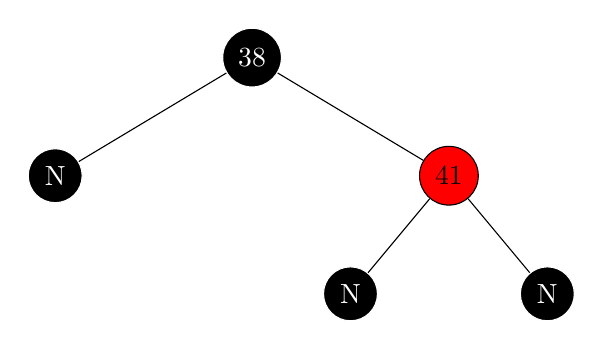
\begin{tikzpicture}[level/.style={sibling distance=50mm/#1}]
\node [circle,draw,color=white, fill=black] (a){38}
	child{node [circle,draw,color=white, fill=black] (k) {N}}
	child{node [circle,draw,color=black, fill=red] (e) {41}
		child{node [circle,draw,color=white, fill=black] (f) {N}}
		child{node [circle,draw,color=white, fill=black] (g) {N}}};
\end{tikzpicture}\\

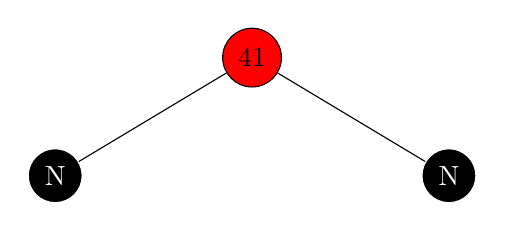
\begin{tikzpicture}[level/.style={sibling distance=50mm/#1}]
\node [circle,draw,color=black, fill=red] (a){41}
	child{node [circle,draw,color=white, fill=black] (k) {N}}
	child{node [circle,draw,color=white, fill=black] (g) {N}};
\end{tikzpicture}\\



\begin{tikzpicture}[level/.style={sibling distance=50mm/#1}]
\node [circle,draw,color=white, fill=black] (a){N};
\end{tikzpicture}\\

\noindent\textbf{Exercise 13.4-4} \\

Since it is possible that $w$ is T.nil, any line of RB-DELETE-FIXUP(T,x) which examines or modifies $w$ must be included.  However, as described on page 317, $x$ will never be T.nil, so we need not include those lines. \\

\noindent\textbf{ Exercise 13.4-5} \\

Our count will include the root (if it is black).

Case 1: The count to each subtree is 2 both before and after

Case 2: The count to the subtrees $\alpha$ and $\beta$ is 1+count(c) in both cases, and the count for the rest of the subtrees goes from 2+count(c) to 1+count(c). This decrease in the count for the other subtreese is handled by then having $x$ represent an additional black.

Case 3: The count to $\epsilon$ and $\zeta$ is 2+count(c) both before and after, for all the other subtrees, it is 1+count(c) both before and after

Case 4: For $\alpha$ and $\beta$, the count goes from 1+count(c) to 2+count(c). For $\gamma$ and $\delta$, it is 1+count(c)+count(c') both before and after. For $\epsilon$ and $\zeta$, it is 1+ count(c) both before and after. This increase in the count for $\alpha$ and $\beta$ is because $x$ before indicated an extra black.\\
%check cases 2 and 4


\noindent\textbf{Exercise 13.4-6}\\

At the start of case 1 we have set $w$ to be the sibling of $x$.  We check on line 4 that $w.color == red$, which means that the parent of $x$ and $w$ cannot be red.  Otherwise property 4 is violated.  Thus, their concerns are unfounded. \\

\noindent\textbf{ Exercise 13.4-7} \\

Suppose that we insert the elements $3,2,1$ in that order, then, the resulting tree will look like

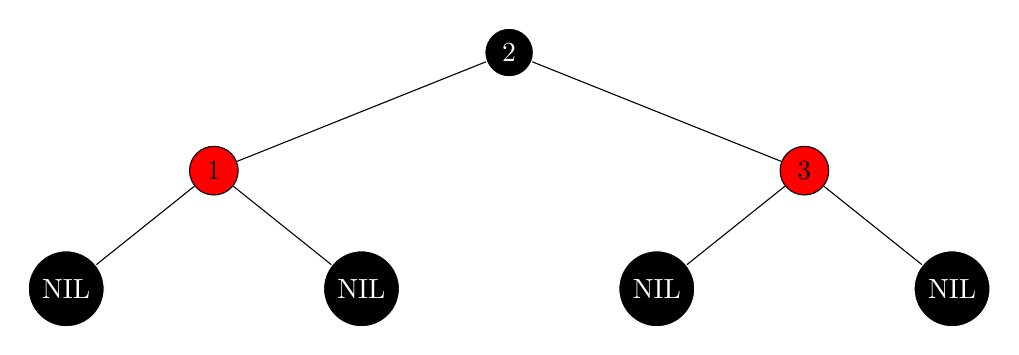
\begin{tikzpicture}[level/.style={sibling distance=75mm/#1}]
\node [circle,draw, color=white, fill = black] (a){2}
  child {
  node [circle,draw,fill = red] (b) {1}
	child{node[circle,draw, color=white, fill = black] (c) {NIL}}
	child{node[circle,draw, color=white, fill = black] (d) {NIL}}
    }
  child{ node [circle,draw,fill =red] (e) {3}
  	child{node[circle,draw, color=white, fill = black] (f) {NIL}}
	child{node[circle,draw, color=white, fill = black] (g) {NIL}}
};
\end{tikzpicture}
Then, after deleting 1, which was the last element added, the resulting tree is 

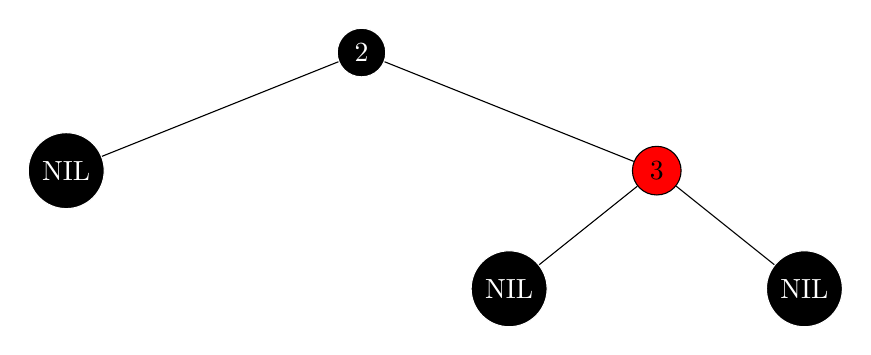
\begin{tikzpicture}[level/.style={sibling distance=75mm/#1}]
\node [circle,draw, color=white, fill = black] (a){2}
 	child{node[circle,draw, color=white, fill = black] (d) {NIL}}    
  child{ node [circle,draw,fill =red] (e) {3}
  	child{node[circle,draw, color=white, fill = black] (f) {NIL}}
	child{node[circle,draw, color=white, fill = black] (g) {NIL}}
};
\end{tikzpicture}

however, the tree we had before we inserted 1 in the first place was 

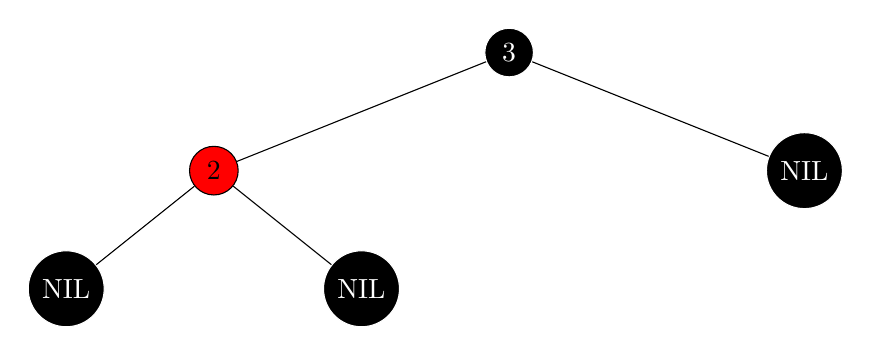
\begin{tikzpicture}[level/.style={sibling distance=75mm/#1}]
\node [circle,draw, color=white, fill = black] (a){3}
  child{ node [circle,draw,fill =red] (e) {2}
  	child{node[circle,draw, color=white, fill = black] (f) {NIL}}
	child{node[circle,draw, color=white, fill = black] (g) {NIL}}
	}
 	child{node[circle,draw, color=white, fill = black] (d) {NIL}};
\end{tikzpicture}

These two red black trees are clearly different

\noindent\textbf{ Problem 13-1} \\

\begin{enumerate}[a.]
\item
We need to make a new version of every node that is an ancestor of the node that is inserted or deleted.

\item
See the algorithm, PERSISTENT-TREE-INSERT

\begin{algorithm}
\caption{PERSISTENT-TREE-INSERT(T,k)}
\begin{algorithmic}
\State $x = T.root$
\If{x==NIL}
\State T.root = new node(key =k)
\EndIf
\While{$x\neq NIL$}
\State y=x
\If{k<x.key}
\State x=  x.left
\State y.left = copyof(x)
\Else
\State x= x.right
\State y.right = copyof(x)
\EndIf
\EndWhile
\State z = new node(key = k, p = y)
\If{k < y.key}
\State y.left = z
\Else
\State y.right = z
\EndIf
\end{algorithmic}
\end{algorithm}

\item
Since the while loop will only run at most $h$ times, since the distance from $x$ to the root is increasing by 1 each time and bounded by the height. Also, since each iteration only takes a constant amount of time and uses a constant amount of additional space, we have that both the time and space complexity are $O(h)$.


\item
When we insert an element, we need to make a new version of the root. So, any nodes that point to the root must have a new copy made so that they point to the new root. So, all nodes of depth 1 must be copied. Similarly, all nodes that point to those must have new copies so that have the correct version. So, all nodes of depth 2 must be copied. Similarly, all nodes must be copied. So, we have that we need at least $\Omega(n)$ time and additional space.

\item
Since the rebalancing operations can only change ancestors, and children of ancestors we only have to allocate at most $2h$ new nodes for each insertion, since the rest of the tree will be unchanged. This is of course assuming that we don't keep track of the parent pointers. This can be achieved by following the suggestions in 13.3-6 applied to both insert and delete. That is, we perform a search for the element where we store the $O(h)$ elements that are either ancestors or children of ancestors. Since these are the only nodes under consideration when doing the insertion and deletion procedure, then we can know their parents even though we aren't keeping track of the parent pointers for each node. Since the height stays $O(\lg(n))$, then, we have that everything can be done in $O(\lg(n))$.


\end{enumerate}

\noindent\textbf{Problem 13-2}\\
\begin{enumerate}[a.]
\item When we call insert or delete we modify the black-height of the tree by at most 1 and we can modify it according to which case we're in, so no additional storage is required. When descending through $T$, we can determine the black-height of each node we visit in $O(1)$ time per node visited.  Start by determining the black height of the root in $O(\log n)$ time.  As we move down the tree, we need only decrement the height by 1 for each black node we see to determine the new height which can be done in $O(1)$.  Since there are $O(\log n)$ nodes on the path from root to leaf, the time per node is constant. \\

 \item Find the black-height of $T_1$ in $O(\log n)$ time. Then find the black-height of $T_2$ in $O(\log n)$ time.  Finally, set $z = T_1.root$.  While the black height of $z$ is strictly greater than $T_2.bh$, update $z$ to be $z.right$ if such a child exists, otherwise update $z$ to be $z.left$.  Once the height of $z$ is equal to $T_2.bh$, set $y$ equal to $z$.  The runtime of the algorithm is $O(\log n)$ since the height of $T_1$, and hence the number of iterations of the while-loop, is at most $O(\log n)$.\\

\item Let $T$ denote the desired tree.  Set $T.root = x$, $x.left = y$, $y.p = x$, $x.right = T_2.root$ and $T_2.root.p = x$.  Every element of $T_y$ is in $T_1$ which contains only elements smaller than $x$ and every element of $T_2$ is larger than $x$.  Since $T_y$ and $T_2$ each have the binary search tree property, $T$ does as well. \\

\item Color $x$ red.  Find $y$ in $T_1$, as in part b, and form $T = T_y \cup \{ x \} \cup T_2$ as in part c in constant time.  Call T' = RB-TRANSPLANT(T,y,x).  We have potentially violated the red black property if $y$'s parent was red.  To remedy this, call RB-INSERT-FIXUP(T', x).\\

\item In the symmetric situation, simply reverse the roles of $T_1$ and $T_2$ in parts b through d. \\

\item  If $T_1.bh \geq T_2.bh$, run the steps outlined in part d.  Otherwise, reverse the roles of parts $T_1$ and $T_2$ in d and then proceed as before.  Either way, the algorithm takes $O(\log n)$ time because RB-INSERT-FIXUP is $O(\log n)$.

\end{enumerate}

\noindent\textbf{ Problem 13-3} \\

\begin{enumerate}[a.]
\item
Let $T(h)$ denote the minimum size of an AVL tree of height $h$.  Since it is height $h$, it must have the max of it's children's heights is equal to $h-1$. Since we are trying to get as few notes total as possible, suppose that the other child has as small of a height as is allowed. Because of the restriction of AVL trees, we have that the smaller child must be at least one less than the larger one, so, we have that $T(h) \ge T(h-1) + T(h-2) +1$ where the +1 is coming from counting the root node. We can get inequality in the opposite direction by simply taking a tree that achieves the minimum number of number of nodes on height $h-1$ and on $h-2$ and join them together under another node. So, we have that $T(h) = T(h-1)+T(h-2)+1$. Also, $T(0) = 0$, $T(1) = 1$. This is both the same recurrence and initial conditions as the Fibonacci numbers. So, recalling equation (3.25), we have that
\[
T(h) = \left\lfloor \frac{\phi^h}{\sqrt{5}} +\frac{1}{2} \right\rfloor \le n
\]

Rearranging for $h$, we have
\begin{align*}
\frac{\phi^h}{\sqrt{5}} -\frac{1}{2}  &\le n\\
\phi^h  &\le\sqrt{5}\left( n + \frac{1}{2} \right)\\
h &\le \frac{\lg(\sqrt{5}) + \lg(n + \frac{1}{2})}{\lg(\phi)} \in O(\lg(n))
\end{align*}

\item
Let UNBAL(x) denote x.left.h - x.right.h. Then, the algorithm BALANCE does what is desired. Note that because we are only rotating a single element at a time, the value of UNBAL(x) can only change by at most 2 in each step. Also, it must eventually start to change as the tree that was shorter becomes saturated with elements. We also fix any breaking of the AVL property that rotating may of caused by our recursive calls to the children.
\begin{algorithm}
\caption{BALANCE(x)}
\begin{algorithmic}
\While{$|UNBAL(x)| >1$}
\If{$UNBAL(x) >0$}
\State RIGHT-ROTATE(T,x)
\Else
\State LEFT-ROTATE(T,x)
\EndIf
\State BALANCE(x.left)
\State BALANCE(x.right)
\EndWhile
\end{algorithmic}
\end{algorithm}


\item
For the given algorithm AVL-INSERT(x,z), it correctly maintains the fact that it is a BST by the way we search for the correct spot to insert $z$. Also, we can see that it maintains the property of being AVL, because after inserting the element, it checks all of the parents for the AVL property, since those are the only places it could of broken. It then fixes it and also updates the height attribute for any of the nodes for which it may of changed.
\begin{algorithm}
\caption{AVL-INSERT(x,z)}
\begin{algorithmic}
\State w = x
\While{$w\neq NIL$}
\State y = w
\If{$z.key > y.key$}
\State w= w.right
\Else
\State w = w.left
\EndIf
\EndWhile
\State
\If{$z.key > y.key$}
\State y.right = z
\If{y.left = NIL}
\State y.h = 1
\EndIf
\Else
\State y.left = z
\If{y.right = NIL}
\State y.h = 1
\EndIf
\EndIf
\While{$y\neq x$}
\State $y.h = 1 + \max\{y.left.h,y.right.h\}$
\If{$y.left.h > y.right.h +1$}
\State RIGHT-ROTATE(T,y)
\EndIf
\If{$y.right.h > y.left.h +1$}
\State LEFT-ROTATE(T,y)
\State y= y.p
\EndIf
\EndWhile
\end{algorithmic}
\end{algorithm}

\item
Since both for loops only run for $O(h) = O(\lg(n))$ iterations, we have that that is the runtime. Also, only a single rotation will occur in the second while loop because when we do it, we will be decreasing the height of the subtree rooted there, which means that it's back down to what it was before, so all of it's ancestors will have unchanged heights, so, no further balancing will be required.


\end{enumerate}


\noindent\textbf{Problem 13-4}\\
\begin{enumerate}[a.]
\item The root $r$ is uniquely determined because it must contain the smallest priority.  Then we partition the set of nodes into those which have key values less than $r$ and those which have values greater than $r$.  We must make a treap out of each of these and make them the left and right children of $r$.  By induction on the number of nodes, we see that the treap is uniquely determined. \\

\item  Since choosing random priorities corresponds to inserting in a random order, the expected height of a treap is the same as the expected height of a randomly built binary search tree, $\Theta(\log n)$. \\

\item First insert a node as usual using the binary-search-tree insertion procedure.  Then perform left and right rotations until the parent of the inserted node no longer has larger priority. \\

\item The expected runtime of TREAP-INSERT is $\Theta(\log n)$ since the expected height of a treap is $\Theta(\log n)$.\\

\item To insert $x$, we initially run the BST insert procedure, so $x$ is a leaf node.  Every time we perform a left rotation, we increase the length of the right spine of the left subtree by 1.  Every time we perform a right rotation, we increase the length of the left spine of the right subtree by 1. Since we only perform left and right rotations, the claim follows. \\

\item If $X_{ik} = 1$ then the properties must hold by the binary-search-tree property and the definition of treap.  On the other hand, suppose $y.key < z.key < x.key$ implies $y.priority < z.priority$.  If $y$ wasn't a child of $x$ then taking $z$ to be the lowest common ancestor of $x$ and $y$ would violate this.  Since $y.priority > x.priority$,$y$ must be a child of $x$.  Since $y.key < x.key$, $y$ is in the left subtree of $x$.  If $y$ is not in the right spine of the left subtree of $x$ then there must exist some $z$ such that $y.priority > z.priority > x.priority$ and $y.key < z.key <x.key$, a contradiction. \\

\item We need to compute the probability that the conditions of part f are satisfied. For all $z \in [i+1, k-1]$ we must have $x.priority < y.priority < z.priority$.  There are $(k-i-1)!$ ways to permute the priorities corresponding to these $z$, out of $(k-i+1)!$ ways to permute the priorities corresponding to all elements in $[i,k]$.  Cancellation gives $P\{X_{ik}\} = \frac{1}{(k-i+1)(k-i)}$. \\

\item We use part g then simplify the telescoping series:
\begin{align*}
E[C] &= \sum_{j=1}^{k-1} E[X_{jk}] \\
&= \sum_{j=1}^{k-1} \frac{1}{(k-j+1)(k-j)}\\
&= \sum_{j=1}^{k-1}\frac{1}{j(j+1)} \\
&= \sum_{j=1}^{k-1}\frac{1}{j} - \frac{1}{j+1} \\
&= 1 - \frac{1}{k}.
\end{align*}

\item A node $y$ is in the left spine of the right subtree of $x$ if and only if it would be in the right spine of the left subtree of $x$ in the treap where every node with key $k$ is replaced by a node with key $n-k$.  Replacing $k$ by $n-k$ in the expectation computation of part h gives the result. \\

\item  By part e, the number of rotations is $C + D$.  By linearity of expectation, $E[C+D] = 2 - \frac{1}{k} - \frac{1}{n-k+1} \leq 2$ for any choice of $k$.

\end{enumerate}

\end{document} 